\documentclass{article}

\usepackage{listings}
\usepackage{parskip}
\setlength{\parskip}{0pt}
\usepackage{graphicx}
\graphicspath{{./images/}}
\usepackage{float}
\usepackage[a4paper, margin=2cm]{geometry}

\title{Pd-Ofelia suficiente para começar}
\author{Gabriel Haruo}
\date{}

\begin{document}

\maketitle

% \section{Introdução}

% \section{Objeto \texttt{ofelia function}}

% \section{Objeto \texttt{ofelia define}}

A biblioteca Ofelia permite que scripts Lua sejam executados no Pure Data.

\section{Sintaxe básica de Lua para Pure Data}

\subsection{Comentários}

Comentários em Lua são iniciados com \texttt{--} e vão até o final da linha.

\begin{center}
  \begin{lstlisting}
  - - Isso e um comentario
  \end{lstlisting}
\end{center}

\subsection{Variáveis}

Variáveis em Lua são definidas com a palavra-chave \texttt{local}.

\begin{center}
  \begin{lstlisting}
  local x = 10
  \end{lstlisting}
\end{center}

\subsubsection{Escopo de variáveis}

Ao declarar uma variável no topo de um script, ela será global e poderá ser acessada por qualquer função no script.

Ao declarar uma variável dentro de uma função, ela será local e só poderá ser acessada dentro da função.

\begin{center}
  \begin{lstlisting}
  local x = 10

  function minhaFuncao()
    local y = 20
    print('Consigo imprimir a variavel x: ' .. x)
    print('Consigo imprimir a variavel y: ' .. y)
  end

  print('Consigo imprimir a variavel x: ' .. x)
  print('Nao consigo imprimir a variavel y: ' .. y)
  \end{lstlisting}
\end{center}

\subsection{Funções}

Funções em Lua são definidas com a palavra-chave \texttt{function}.

\begin{center}
  \begin{lstlisting}
  function minhaFuncao()
    print('Executei a funcao minhaFuncao!')
  end
  \end{lstlisting}
\end{center}

\subsubsection{Parâmetros de entrada}

Parâmetros de entrada são definidos entre parênteses.

\begin{center}
  \begin{lstlisting}
  function minhaFuncaoComParametro(x)
    print('Executei a funcao minhaFuncaoComParametro')
    print(' com o parametro ' .. x)
  end
  \end{lstlisting}
\end{center}

\subsection{Listas}

Listas em Lua são definidas entre chaves.
Para acessar um elemento da lista, use o índice do elemento entre colchetes.

\textbf{Obs.:} As listas em Lua são indexadas a partir de 1.

\begin{center}
  \begin{lstlisting}
  local lista = {10, 20, 30}
  print('Primeiro elemento da lista: ' .. lista[1])
  \end{lstlisting}
\end{center}

\subsection{Laços}

Laços em Lua são definidos com as palavras-chave \texttt{for}, \texttt{do} e \texttt{end}.

\begin{center}
  \begin{lstlisting}
  for i=1, 10 do
    print(i)
  end
  \end{lstlisting}
\end{center}

\subsection{Estruturas condicionais}

Estruturas condicionais em Lua são definidas com as palavras-chave \texttt{if}, \texttt{else}, \texttt{elseif}, \texttt{then}, e \texttt{end}.
Use \texttt{and} e \texttt{or} para combinar condições.

\begin{center}
  \begin{lstlisting}
  local x = 10

  if x > 5 then
    print('x e maior que 5')
  elseif x < 5 then
    print('x e menor ou igual a 5')
  else
    print('x e igual a 5')
  end
  \end{lstlisting}
\end{center}

\section{Executando scripts \texttt{.lua} no Pure Data}

A biblioteca Ofelia registra automaticamente funções nomeadas como \texttt{ofelia.*} para serem usadas como \textbf{manipuladores de mensagens} no Pure Data.

Vamos exemplificar como isso funciona.
Crie um arquivo \texttt{meuScript.lua} e defina a seguinte função:

\begin{center}
  \begin{lstlisting}
  function ofelia.minhaMensagem()
    print('Executei a funcao minhaMensagem!')
  end
  \end{lstlisting}
\end{center}

Crie um patch em Pure Data nomeado \texttt{meuPatch.pd} no mesmo diretório do script e adicione os seguintes objetos:

\begin{figure}[h]
  \centering
  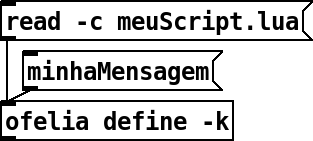
\includegraphics[width=100pt]{passo1.png}
\end{figure}

Clique na mensagem \texttt{read -c meuScript.lua} para carregar o script no Pure Data. Agora, clique na mensagem \texttt{minhaMensagem} para \textbf{executar a função do script com o nome da mensagem mandada}. A função \texttt{ofelia.minhaMensagem()} será executada e a mensagem \texttt{Executei a funcao minhaMensagem!} será impressa no console.

\subsection{\texttt{ofelia.bang()}}

Para executar uma função ao clicar em um objeto \texttt{bang}, é necessário adicionar um objeto \texttt{bang} ao patch e definir a função \texttt{ofelia.bang()} no script.

\begin{figure}[H]
  \centering
  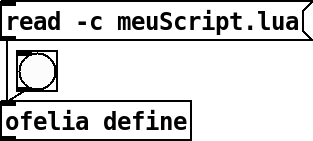
\includegraphics[width=100pt]{bang.png}
\end{figure}

Adicione a seguinte função ao script \texttt{meuScript.lua}:

\begin{center}
  \begin{lstlisting}
  function ofelia.bang()
    print('Executei a funcao ao ativar o bang!')
  end
  \end{lstlisting}
\end{center}

Agora, ao clicar no objeto \texttt{bang}, a função \texttt{ofelia.bang()} será executada e a mensagem \texttt{Executei a funcao ao ativar o bang!} será impressa no console.

\subsection{\texttt{ofelia.list(lista)}}

Para executar uma função ao enviar uma lista de valores, é necessário adicionar uma mensagem com sua lista ao patch e definir a função \texttt{ofelia.list()} no script.

\begin{figure}[H]
  \centering
  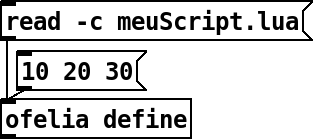
\includegraphics[width=100pt]{list.png}
\end{figure}

Adicione a seguinte função ao script \texttt{meuScript.lua}:

\begin{center}
  \begin{lstlisting}
  function ofelia.list(lista)
    print('Executei a funcao ao enviar uma lista de valores!')
    for i=1, #lista do
      print('Valor ' .. i .. ' da lista: ' .. lista[i])
    end
  end
  \end{lstlisting}
\end{center}

Agora, ao enviar a mensagem \texttt{10 20 30}, a função \texttt{ofelia.list()} será executada e as mensagens \texttt{Executei a funcao ao enviar uma lista de valores!}, \texttt{Valor 1 da lista: 10}, \texttt{Valor 2 da lista: 20} e \texttt{Valor 3 da lista: 30} serão impressas no console.

\subsection{\texttt{ofelia.perform(bloco)}}

Para executar uma função a cada ciclo DSP, é necessário definir a função \texttt{ofelia.perform()} no script.
Em seu patch, adicione um objeto \texttt{ofelia define} com a flag \texttt{-s11}. Essa flag indica que o objeto possui 1 entrada de sinal e 1 saída de sinal.

\begin{figure}[H]
  \centering
  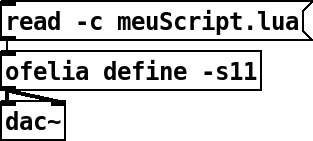
\includegraphics[width=100pt]{perform.png}
\end{figure}

A função \texttt{ofelia.perform()} recebe um vetor de 64 amostras como parâmetro, que deve ser preenchido com as amostras de saída e retornado.
Vamos preencher o bloco de amostras com um ruído branco. Para isso, adicione a seguinte função no script \texttt{meuScript.lua}:

\begin{center}
  \begin{lstlisting}
  function ofelia.perform(bloco)
    for i=1, 64 do
      bloco[i] = 2*math.random() - 1
    end
    return bloco
  end
  \end{lstlisting}
\end{center}

Abaixe o volume! Pois ao conectar o objeto \texttt{ofelia define -s11} a um objeto \texttt{dac\textasciitilde}, um ruído branco será reproduzido.

% \section{O módulo \texttt{M}}
% % "M" is the name of a module table that exists in each "ofelia define" object which includes built-in functions such as "M.bang()" function. You can add any variables or functions to the module.
% % Perceba que não definimos \texttt{M} em lugar algum em nosso script.
% % Na verdade, \texttt{M} é um módulo-tabela que existe em todo objeto \texttt{ofelia define} e inclui funções embutidas como a função \texttt{M.bang()} (detalhes das funções embutidas podem ser encontradas na sessão \ref{subsection:funcoes-embutidas} deste documento).
% % Além disso, é possível definir variáveis e funções personalizadas no módulo \texttt{M}.

% \subsection{Funções embutidas}\label{subsection:funcoes-embutidas}

% O Ofelia oferece algumas funções embutidas.

% \subsubsection{\texttt{M.*()}}

% Algumas das funções embutidas com o módulo \texttt{M} são:

% \begin{center}
%   \begin{lstlisting}
%   function M.bang()
%     print("got bang")
%   end

%   function M.float(f)
%     print("got float : " .. f)
%     return f
%   end
%   ;
%   function M.symbol(s)
%     print("got symbol : " .. s)
%   end

%   function M.list(l)
%     for i=1, #l do
%       print("got list : " .. l[i])
%     end
%   end
%   \end{lstlisting}
% \end{center}


\end{document}